\documentclass{report}
\usepackage{graphicx}


\begin{document}

\title{\textbf{Homework 1:} Numerical Integration, differentiation, and bisection}
\author{A.L. Phillips\\
  Department of Physics,% Astronomy, and Applied Physics,\\
  Rensselaer Polytechnic Institute\\
  \texttt{philla3@rpi.edu}}
\date{12 February 2013}
\maketitle
\chapter{Integration, differentiation, and bisection}

\section{Background}
\begin{enumerate}
\item To date,Mathematical operations may be conducted analytically or numerically. Analyti....  
\end{enumerate}

\section{Sources of Error}
\begin{enumerate}
\item Roundoff vs Truncation
\\Machine epsilon...
Two sources of error in numerical methods are Round-off and Truncation errors. Round-off errors are the result of systems having a finite quantity of significant figures to represent numbers. For example, if a computer is capable of can store three significant figures, then it could approximate $ \frac{1}{3}$ as $0.333$. Because the computer is not representing $ \frac{1}{3}$ $exactly$ as $0.\overline{3}$, a round-off error ($\xi_{max_{T}}$) occurs. 
\\In this case, $\displaystyle \xi_{max_{T}} = \frac{1}{3} - 0.333 = 0.000\overline{3} $
\\
\\Truncation error is the result of truncating (shortening) a mathematical procedure. In numerical methods, the shortening of a mathematical procedure occurs whenever we are required to approach zero (integrate) or use an infinite number of terms (series). For example, the Maclaurin series expansion of $cos(x) = 1 - \frac{1}{2}x^2 + \frac{1}{24}x^4 - \frac{1}{720}x^6 + \ldots$ .Since we must chose a finite number of terms, a truncation error will ultimately result. If we choose two terms, the truncation error would then equal the sum of all the excluded terms. Namely, $\frac{1}{24}x^4 - \frac{1}{720}x^6 + \ldots$.  

\end{enumerate}

\section{Numerical Integration Techniques}
\begin{enumerate}
\item Trapezoidal Method:
\\
\\
The trapezoid rule calculates the area under a curve much like a Riemann sum. Here, rather than using rectangles, the trapezoidal method employs trapezoids. The graphic below depicts the use of a single trapezoid to approximate the area under the blue curve. The more trapezoids that are added between $a$ and $b$, the closer the "secant-shaped" tops of each trapezoid will become to the tangent on the curve above it.\\
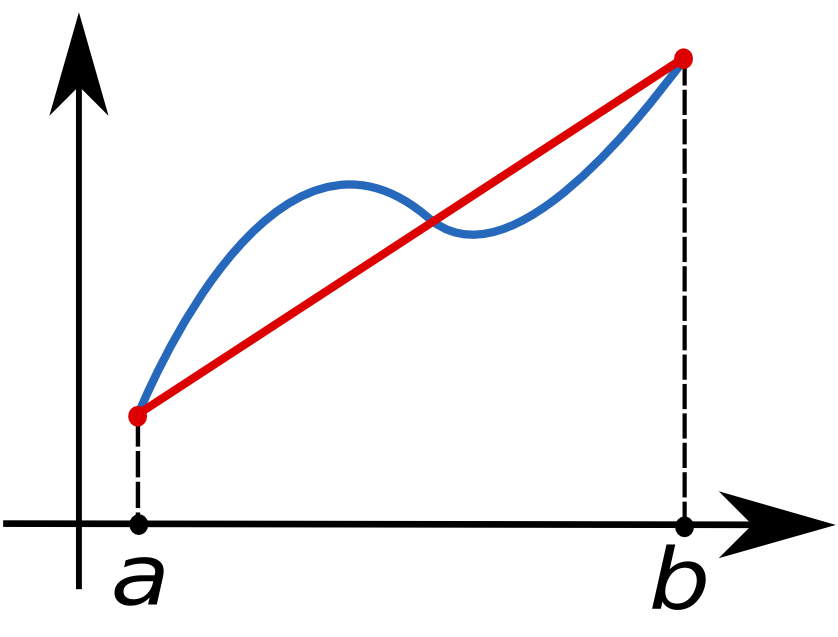
\includegraphics[scale=.15]{trapezoid.png}
\\
\\
The general formula for the approximation of a definite integral via the Trapezoid Rule is as follows:
\\ $\displaystyle \int^b_a f(x)\,dx  \approx  \frac{\Delta x}{2}\Big[f(x_{0})+2f(x_1)+\ldots+2f(x_{n-1})+f(x_n)\Big]$ 
\\where $\displaystyle \Delta x = \frac{(b-a)}{n}$ .......... $\displaystyle x_i = a + i(\frac{b-a}{n})$
\\
\\
\\
\\Trapezoidal Error: 
\\
\\The maximum amount of truncation error ($\xi_{max_{T}}$) when using the trapezoid rule may be determined as follows:
\\
\\$\displaystyle \xi_{max_{T}} = \frac{(b-a)^{3}\left|f^{(2)}_{(max)}\right|}{12n^2}$\\ \\Here, $\displaystyle b$ and $\displaystyle a$ are the upper and lower limits of integration, $\displaystyle n$ is the trapezoid quantity being used and $f^{(2)}_{(max)}$ is the second derivative of the function. The $(max)$ subscript indicates that the second derivative should be evaluated at the point from $\displaystyle [a,b]$ which maximizes the value of $f^{(2)}$.
\\
\\Similarly, the minimum number of trapezoids needed to calculate an integral to within a given accuracy ($\xi_{max}$) may be determined by solving the above equation for $\displaystyle n$: 
\\
\\
$\displaystyle n \geq \sqrt{\frac{(b-a)^{3}\left|f^{(4)}_{(max)}\right|}{12(\xi_{max})}} $
\\Note: $\displaystyle n$ must be a whole number; therefore if $n \geq 10.5$ then choose $n = 11$


\item Simpson's Rule:

\includegraphics[scale=.75]{integration.eps}

\item Gaussian Quadrature:

\item Comparison:

\end{enumerate}


\section{Numerical Differentiation Techniques}
\begin{enumerate}
\item Test
\end{enumerate}

\section{Algorithmic Considerations}
\section{Implementation}
\section{Results}
\section{Discussion}
\section{References}

\section{Original Assignment}
\begin{enumerate}
\item Write a double-precision program to integrate an arbitrary
  function numerically using the trapezoid rule, the Simpson rule, and
  Gaussian quadrature (for GC, limit yourself to a simple 3 point
  approximation within each interval: use one interval only in this case).  In the discussion of your
  results, a plot of the relative error $\epsilon =
  |\frac{\mathrm{numerical-exact}}{\mathrm{exact}}|$ for each approach should be included.
\item Compute the first derivative of $x^2$, $x^3$, $e^{-x}$, and
  another well-behaved, non-trivial, function of your choice, using
  forward difference, central difference, and 5-point approximation.
\begin{enumerate}
\item In each case plot the error as function of step size (consider using
  log-log scales)
\item In your discussion, make sure to talk about the best step size
  to use (Refer to the class notes).
  \item Make sure you consider the particular cases where a given approximation is exact. 
\end{enumerate}

\item Write a C++ program that finds the zero of a function using the bisection method. 
\item (optional, for 2 extra credits) Write a C++ program that finds the zero of a function using the newton-Raphson method. 
\end{enumerate}
The section titles provided below are suggested as guides, feel free to adapt for your own presentation. You do \textbf{not} need to provide listings of your program (but you can if it helps the discussion).


\end{document}
